\documentclass{report}

% Packages
\usepackage{lipsum} % For generating dummy text
\usepackage{graphicx} % For including images
\usepackage{cite} % For citations
\usepackage{hyperref} % For hyperlinks

% Title page information
\title{InfiniTerra: An Infinite Terrain Generation System}
\author{Mirto Randellini}
\date{\today}

\begin{document}

% Title page
\maketitle

% Table of contents
\tableofcontents

% Abstract
\begin{abstract}
This is the abstract of my report.
\end{abstract}

% Introduction
\chapter{Introduction}
\label{ch:introduction}
% Why make an infinite terrain?
Infinite terrains are a common feature in video games and other real-time applications, like flight simulators and virtual reality experiences.
They allow for the creation of vast, open worlds that players can explore without encountering any boundaries.
This can enhance the sense of immersion and freedom in a game, as players can travel in any direction without being constrained by the size of the game world.
In this report, we will discuss the design and implementation of an infinite terrain generation system called InfiniTerra.
We will cover the theory behind terrain generation, the algorithms used to generate the terrain, and the rendering techniques used to display the terrain to the player.
We will also discuss the challenges of creating an infinite terrain system and how they were overcome in the development of InfiniTerra.
% Relevant existing work in games
Before diving into the details of the system, it is interesting to mention some of the existing work in the field of terrain generation.
The earliest use of procedural generation in games can be traced back to the 1980s, with games like \textit{Hack} and \textit{Rogue}.
These games used procedural generation to create dungeons and levels that were different each time the player played the game and they spawned a whole genre of games known as roguelikes.

\begin{figure}[h!]
  \centering
  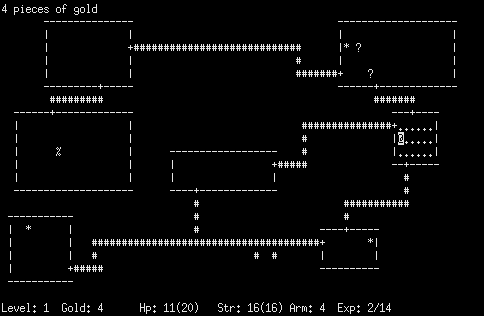
\includegraphics[width=0.75\textwidth]{img/rogue.png}
  \caption{A procedurally generated dungeon map in the videogame Rogue.}
  \label{fig:nethack}
\end{figure}

Moving forward to 1996, the game \textit{Elder Scrolls II: Daggerfall} featured a procedurally generated world with a size of 161,600 square kilometers (approximately the size of England), which was the largest game world ever created at the time, and it is still one of the largest game worlds ever created.
To be precise the wilderness between locations is based on a rudimentary heightmap, one pixel of which covers 800 in-game metres.
Smaller details are randomly generated, while actual locations are pre-generated, and are consequently always the same.

\begin{figure}[h!]
  \centering
  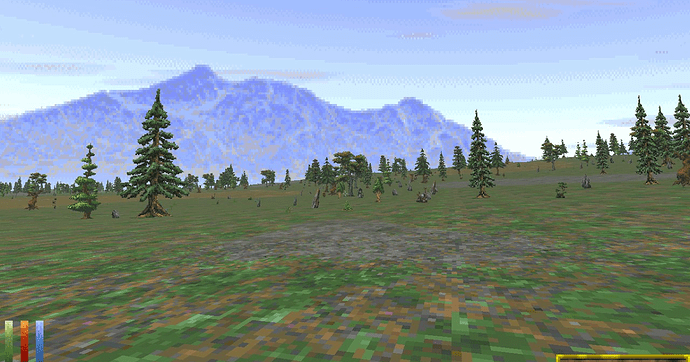
\includegraphics[width=0.75\textwidth]{img/daggerfall.png}
  \caption{The procedurally generated world map of the game Elder Scrolls II: Daggerfall.}
  \label{fig:daggerfall}
\end{figure}

Today one of the most famous examples of procedural generation in games is \textit{Minecraft}, a game that features a procedurally generated world made up of blocks that players can mine and place to create their own structures.
The world in Minecraft is generated using Perlin noise, a type of gradient noise that is commonly used in procedural generation to create natural-looking terrains.
The generation algorithm has then been improved over the years to include more complex features like caves, villages, and biomes.

\begin{figure}[h!]
  \centering
  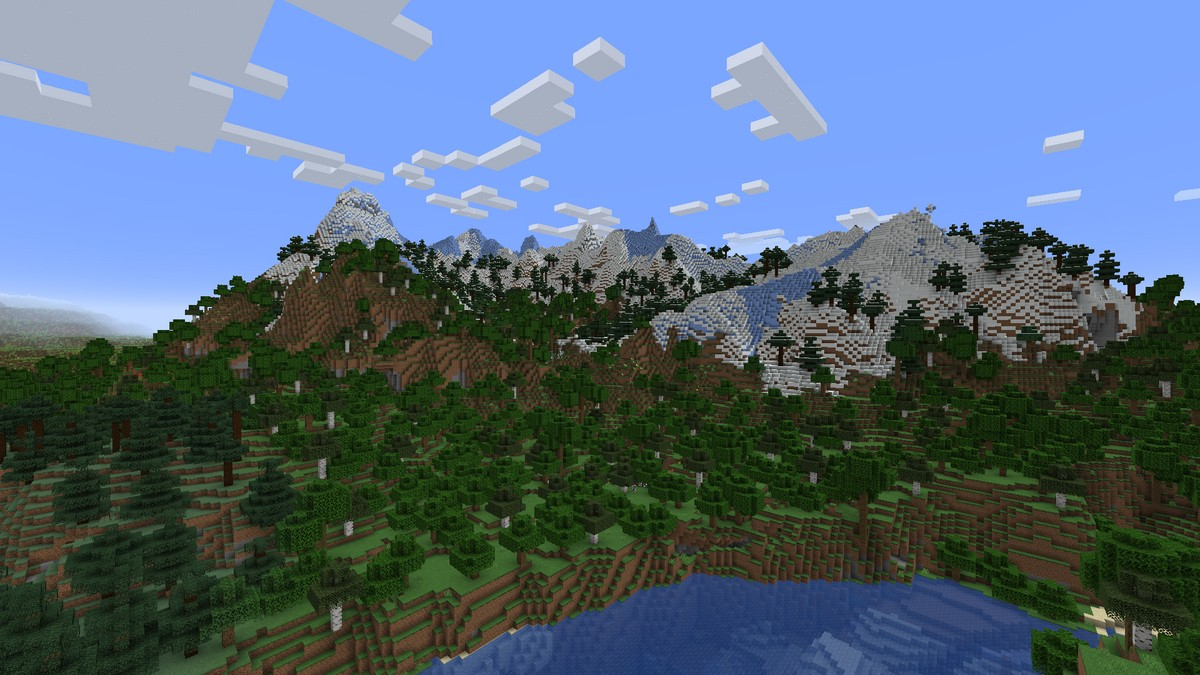
\includegraphics[width=0.75\textwidth]{img/minecraft.jpg}
  \caption{A procedurally generated world in the videogame Minecraft.}
  \label{fig:minecraft}
\end{figure}

%End introduction


\chapter{Generating the terrain}
\label{ch:generating-the-terrain}
% Heightmap generation
Commonly used techniques for terrain generation include heightmap generation, fractal terrain generation, and procedural generation using noise functions.
These techniques use mathematical functions to generate terrain data that can be used to displace the vertices of a grid to create a 3D terrain.
In InfiniTerra, we use a heightmap generation technique based on ridged Perlin noise to create the terrain.
% Perlin noise
Perlin noise is a type of gradient noise developed by Ken Perlin in 1983. It is commonly used in computer graphics to create natural-looking textures and terrains.
Interestingly it's first use was in the movie Tron (1982) to create the light cycle effects.
% CPU implementation
In the first version of the system, the heightmap generation was implemented on the CPU by using the FastNoiseLite library.
This allowed access to a wide variety of noise functions, such as Perlin, Simplex, and Cellular noise, but was not performant enough for generating large terrains.
The generation of a 1024x1024 heightmap took around 5s on a modern CPU, which was too slow for real-time applications.
% GPU implementation (compute shaders)
To improve performance, the heightmap generation was moved to the GPU by using compute shaders.

\subsection*{Compute shaders}

\chapter{Rendering the terrain}
\label{ch:rendering-the-terrain}
% Base geometry (triangles)
% Phong Lighting
\section{Phong Lighting}
% Phong lighting theory
Phong lighting is a shading model developed by Bui Tuong Phong in 1975. It is a local illumination model that approximates the way light interacts with a surface by using three components: ambient, diffuse, and specular.
% Chunking and culling
% LOD (tessellation)
\lipsum[3-4]

% Conclusion
\chapter{Conclusion}
\label{ch:conclusion}
\lipsum[7-8]

% References
\bibliographystyle{plain}
\bibliography{references}

\end{document}